%
% cos2.tex
%
% (c) 2024 Prof Dr Andreas Müller
%
\begin{figure}
\centering
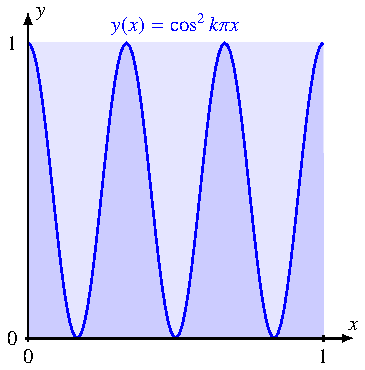
\includegraphics{chapters/050-nebenbedingungen/images/cos2.pdf}
\caption{Berechnung des Integrals von $y(x)=\cos^2 k\pi x$.
Der Graph halbiert das Einheitsquadrat, somit hat das Integral von $y(x)$
den Wert $\frac12$.
\label{buch:nebenbedingungen:aufgabe:501:fig:cos2}}
\end{figure}
